%!TEX root = ../report.tex
\documentclass[report.tex]{subfiles}
\begin{document}
\chapter{Experiment}
In this research and development project, three experiements are being conducted with respected to three use cases: (1) Grasp object by sliding motion along surface and (2) Perform writing task and (3)Resting elbow manipulation . In this chapter, the experiements will be divided according to use cases.
    \section{Setup}
    There are two experiement setups in this research and development project. Use case 1 and 2 share the same set up.
    The common setup is listed below:
    \begin{itemize}
        \item Kinova® Gen3 Ultra lightweight robot maniputlator is attached to a table
        \item A Robotiq 2F-85 gripper is attached to the 7th joint of the Kinova arm
        \item The Kinova arm is connect to a laptop with LAN cable
        \item A Xbox controller
    \end{itemize}
    \paragraph{\large{The setup of use case 1}\\}
    Figure \ref{fig:us1_init} shows the initial pose of the robot arm for both use case 1. To ensure that the robot consistently begins each trial run from its precise starting position, it is necessary to press the B button on the Xbox controller. The motion will starts at a fixed starting pose $q = \{6.28318,0.261895,3.14159,4.01417,0,\\0.959856,0.57079\}$ in radian.
    \begin{figure}[!h]
        \centering
        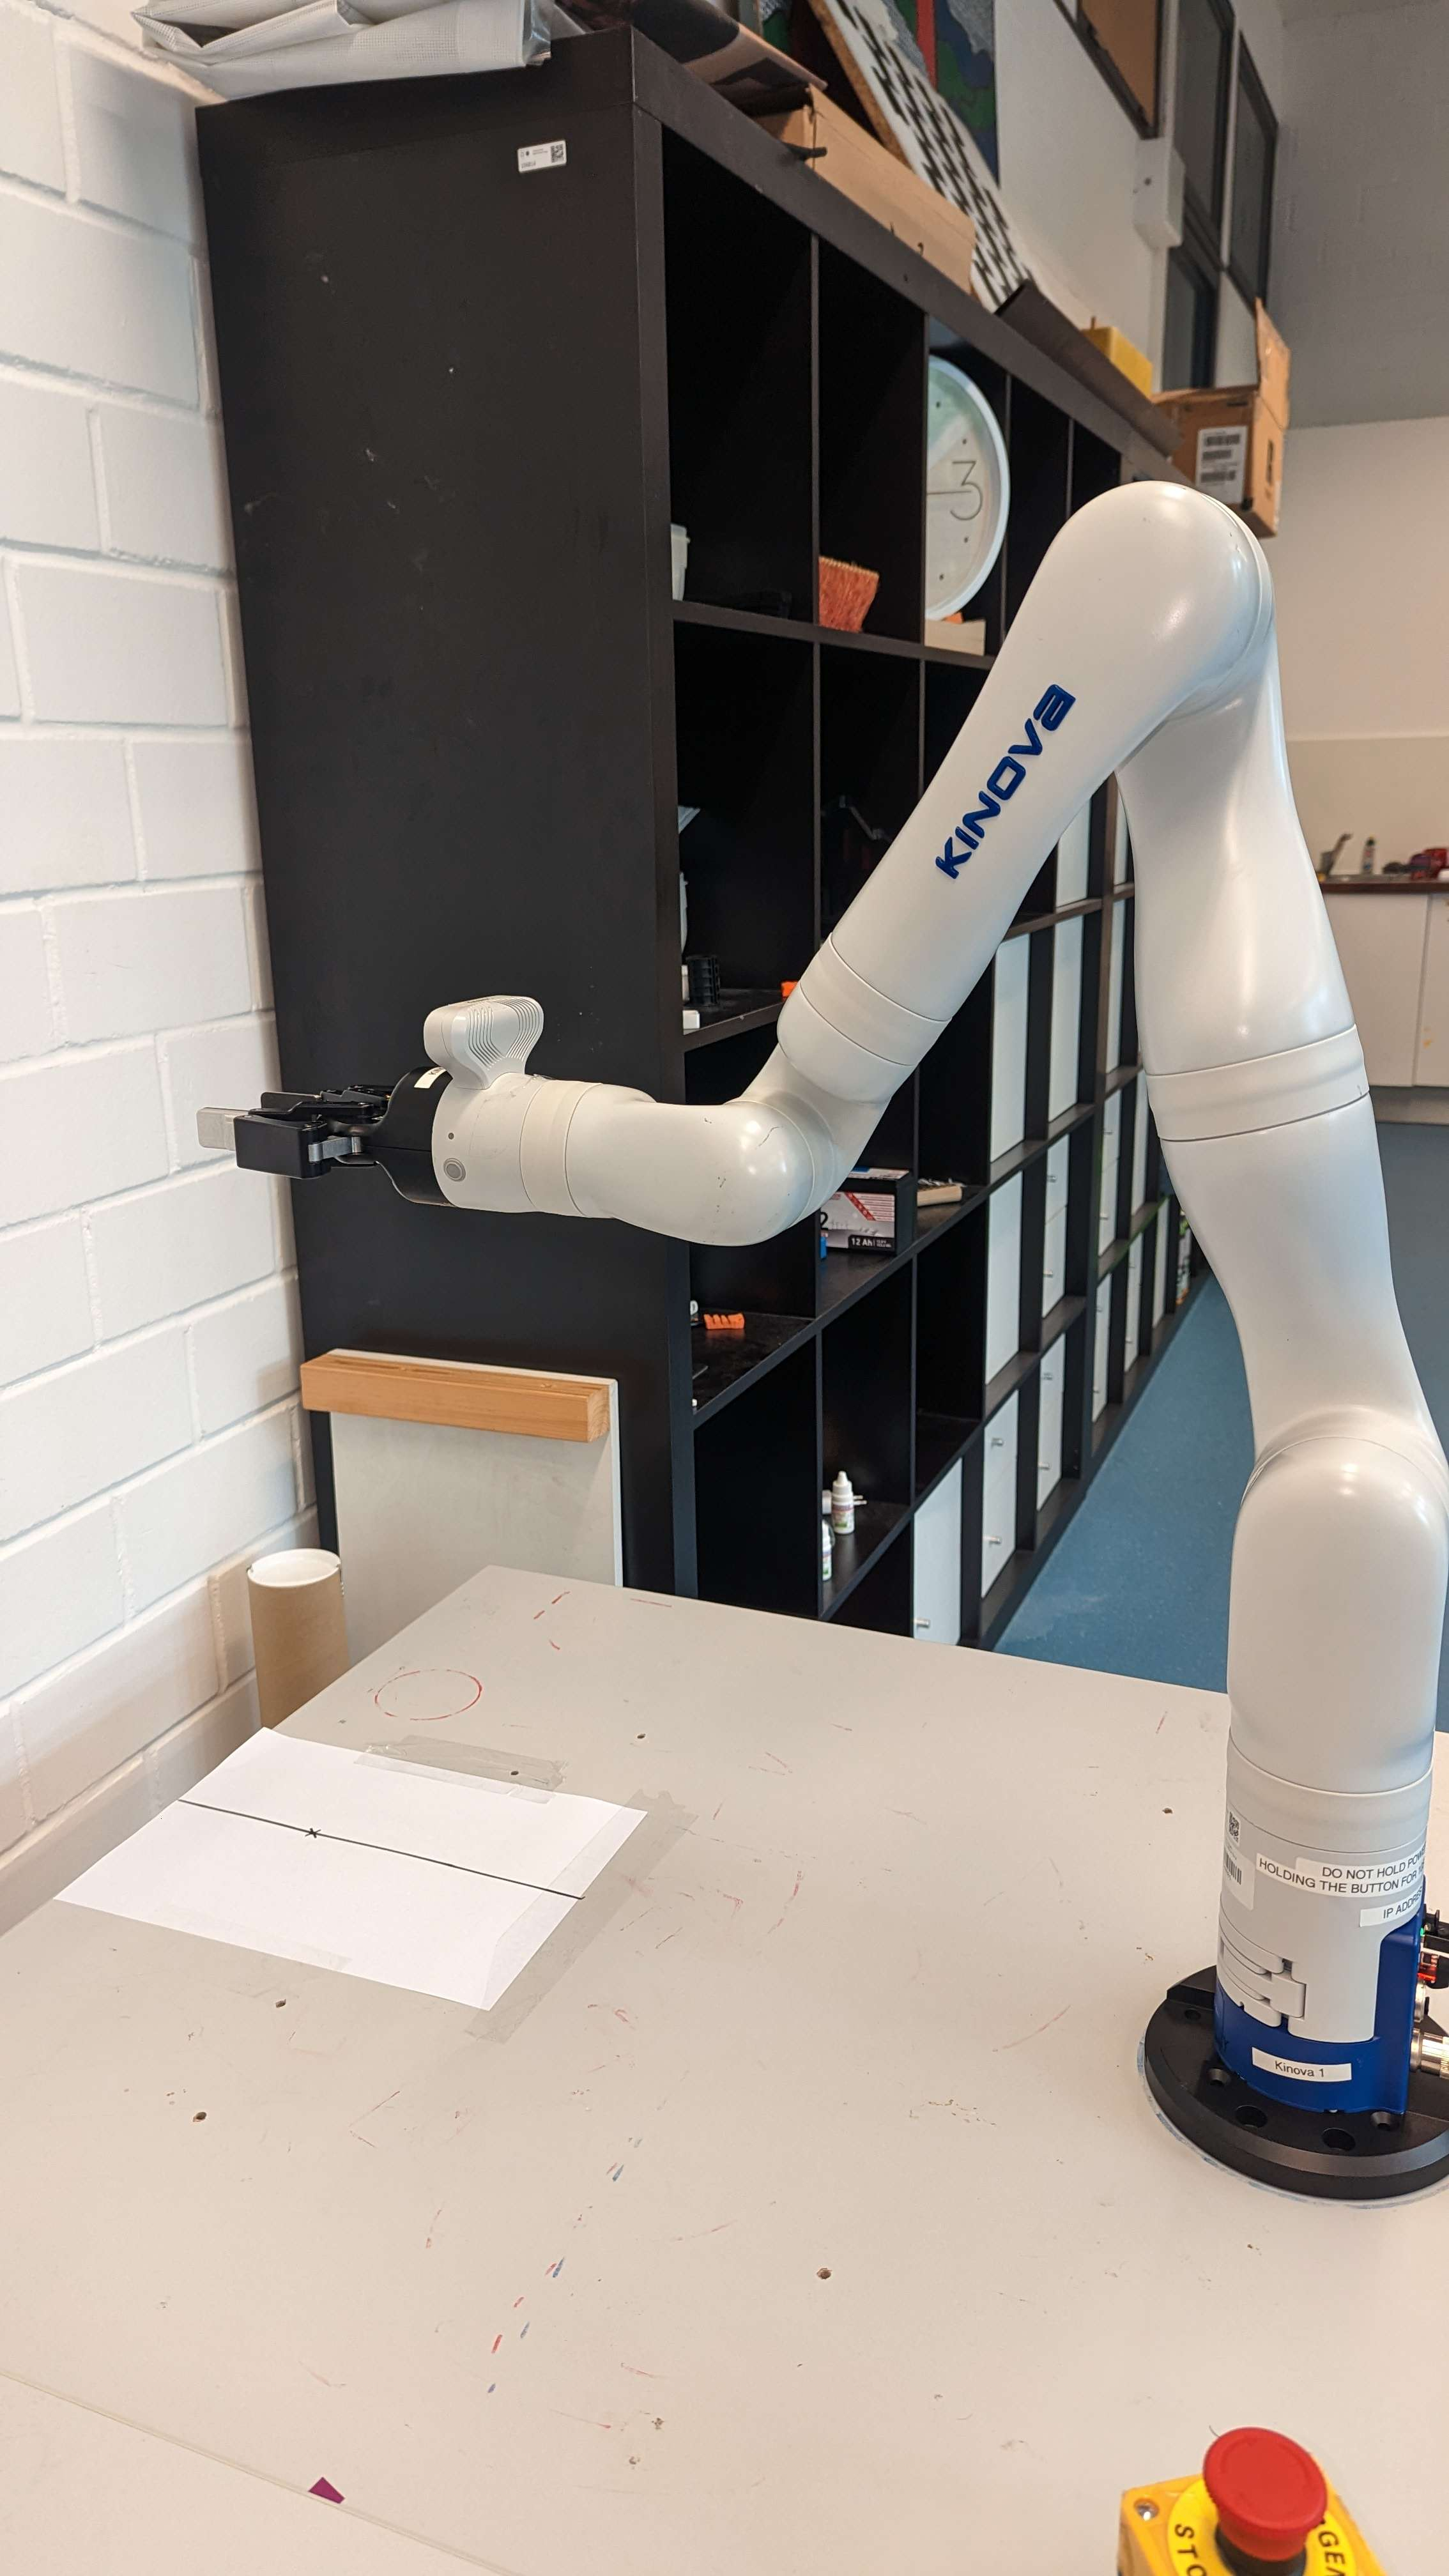
\includegraphics[width=0.3\linewidth]{images/us1_initial.jpg}
        \caption{The initial pose of the robot arm for both use case 1 and 2}
        \label{fig:us1_init}
    \end{figure}
    \paragraph{\large{The setup of use case 2}\\}
    Considering that the purpose of this use case is to perform a writing task, it's important to note that, similar to human writing, the writing motion does not commence from mid-air initially. Instead, the writing task initiates when the tip of the marker pen makes contact with a designated starting reference point on the paper as figure \ref{fig:us2_pen} demostrates. In this particular use case, we will conduct two experiments. In the first experiment, we will establish contact before proceeding with the writing task, whereas in the second experiment, no contact will be established beforehand. Figure \ref{fig:us2_init_con} and \ref{fig:us2_init_nocon} show the initial set up of both experiements. In \ref{fig:us2_init_nocon}, The ruler indicates that the distance from the center of the gripper to the table surface is 10 cm. This measurement serves as the initial height for the writing motion in situations where there is no physical contact with the table.
    \begin{figure}[!h]
        \centering
        \captionsetup[figure]{justification=centering}
        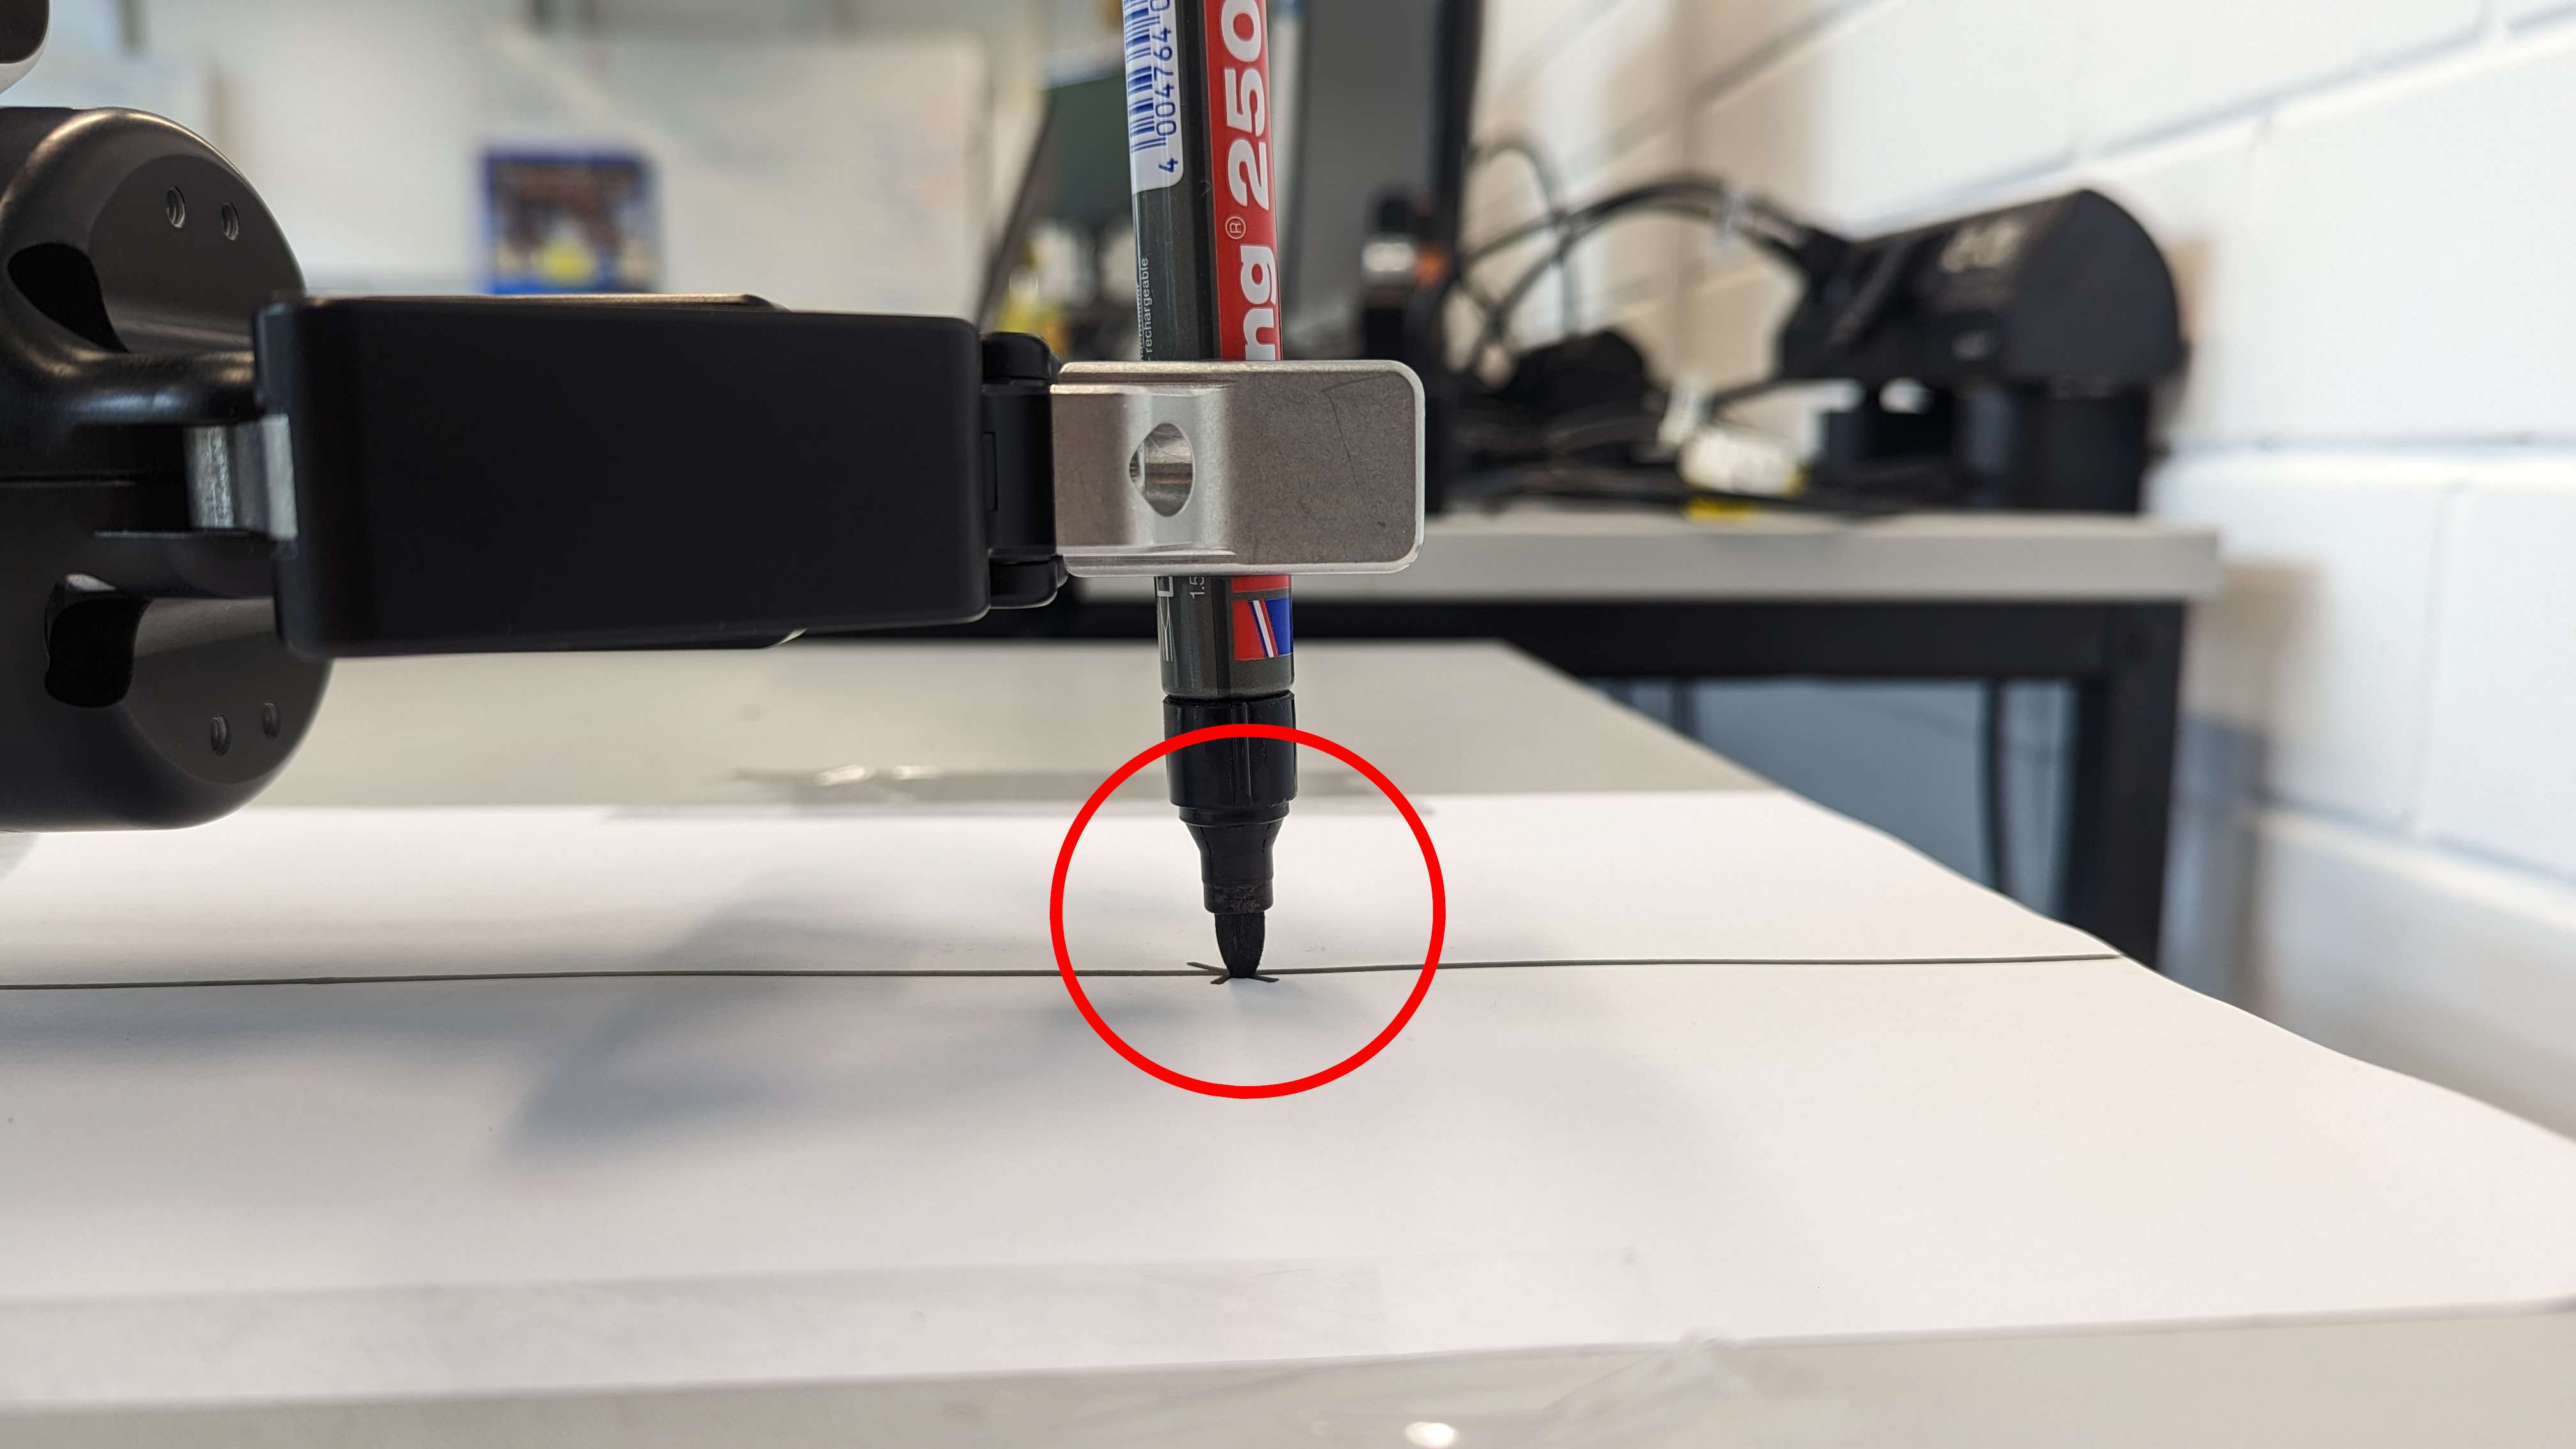
\includegraphics[width=0.9\linewidth]{images/us2_starting_circle.jpg}
        \caption{The tip of the marker pen touches the starting reference point, indicates the robot arm is at the stating position}
        \label{fig:us2_pen}
    \end{figure}
    \begin{figure}[h!]
    \captionsetup[subfigure]{justification=centering}
    \begin{subfigure}{0.5\textwidth}
            \centering
            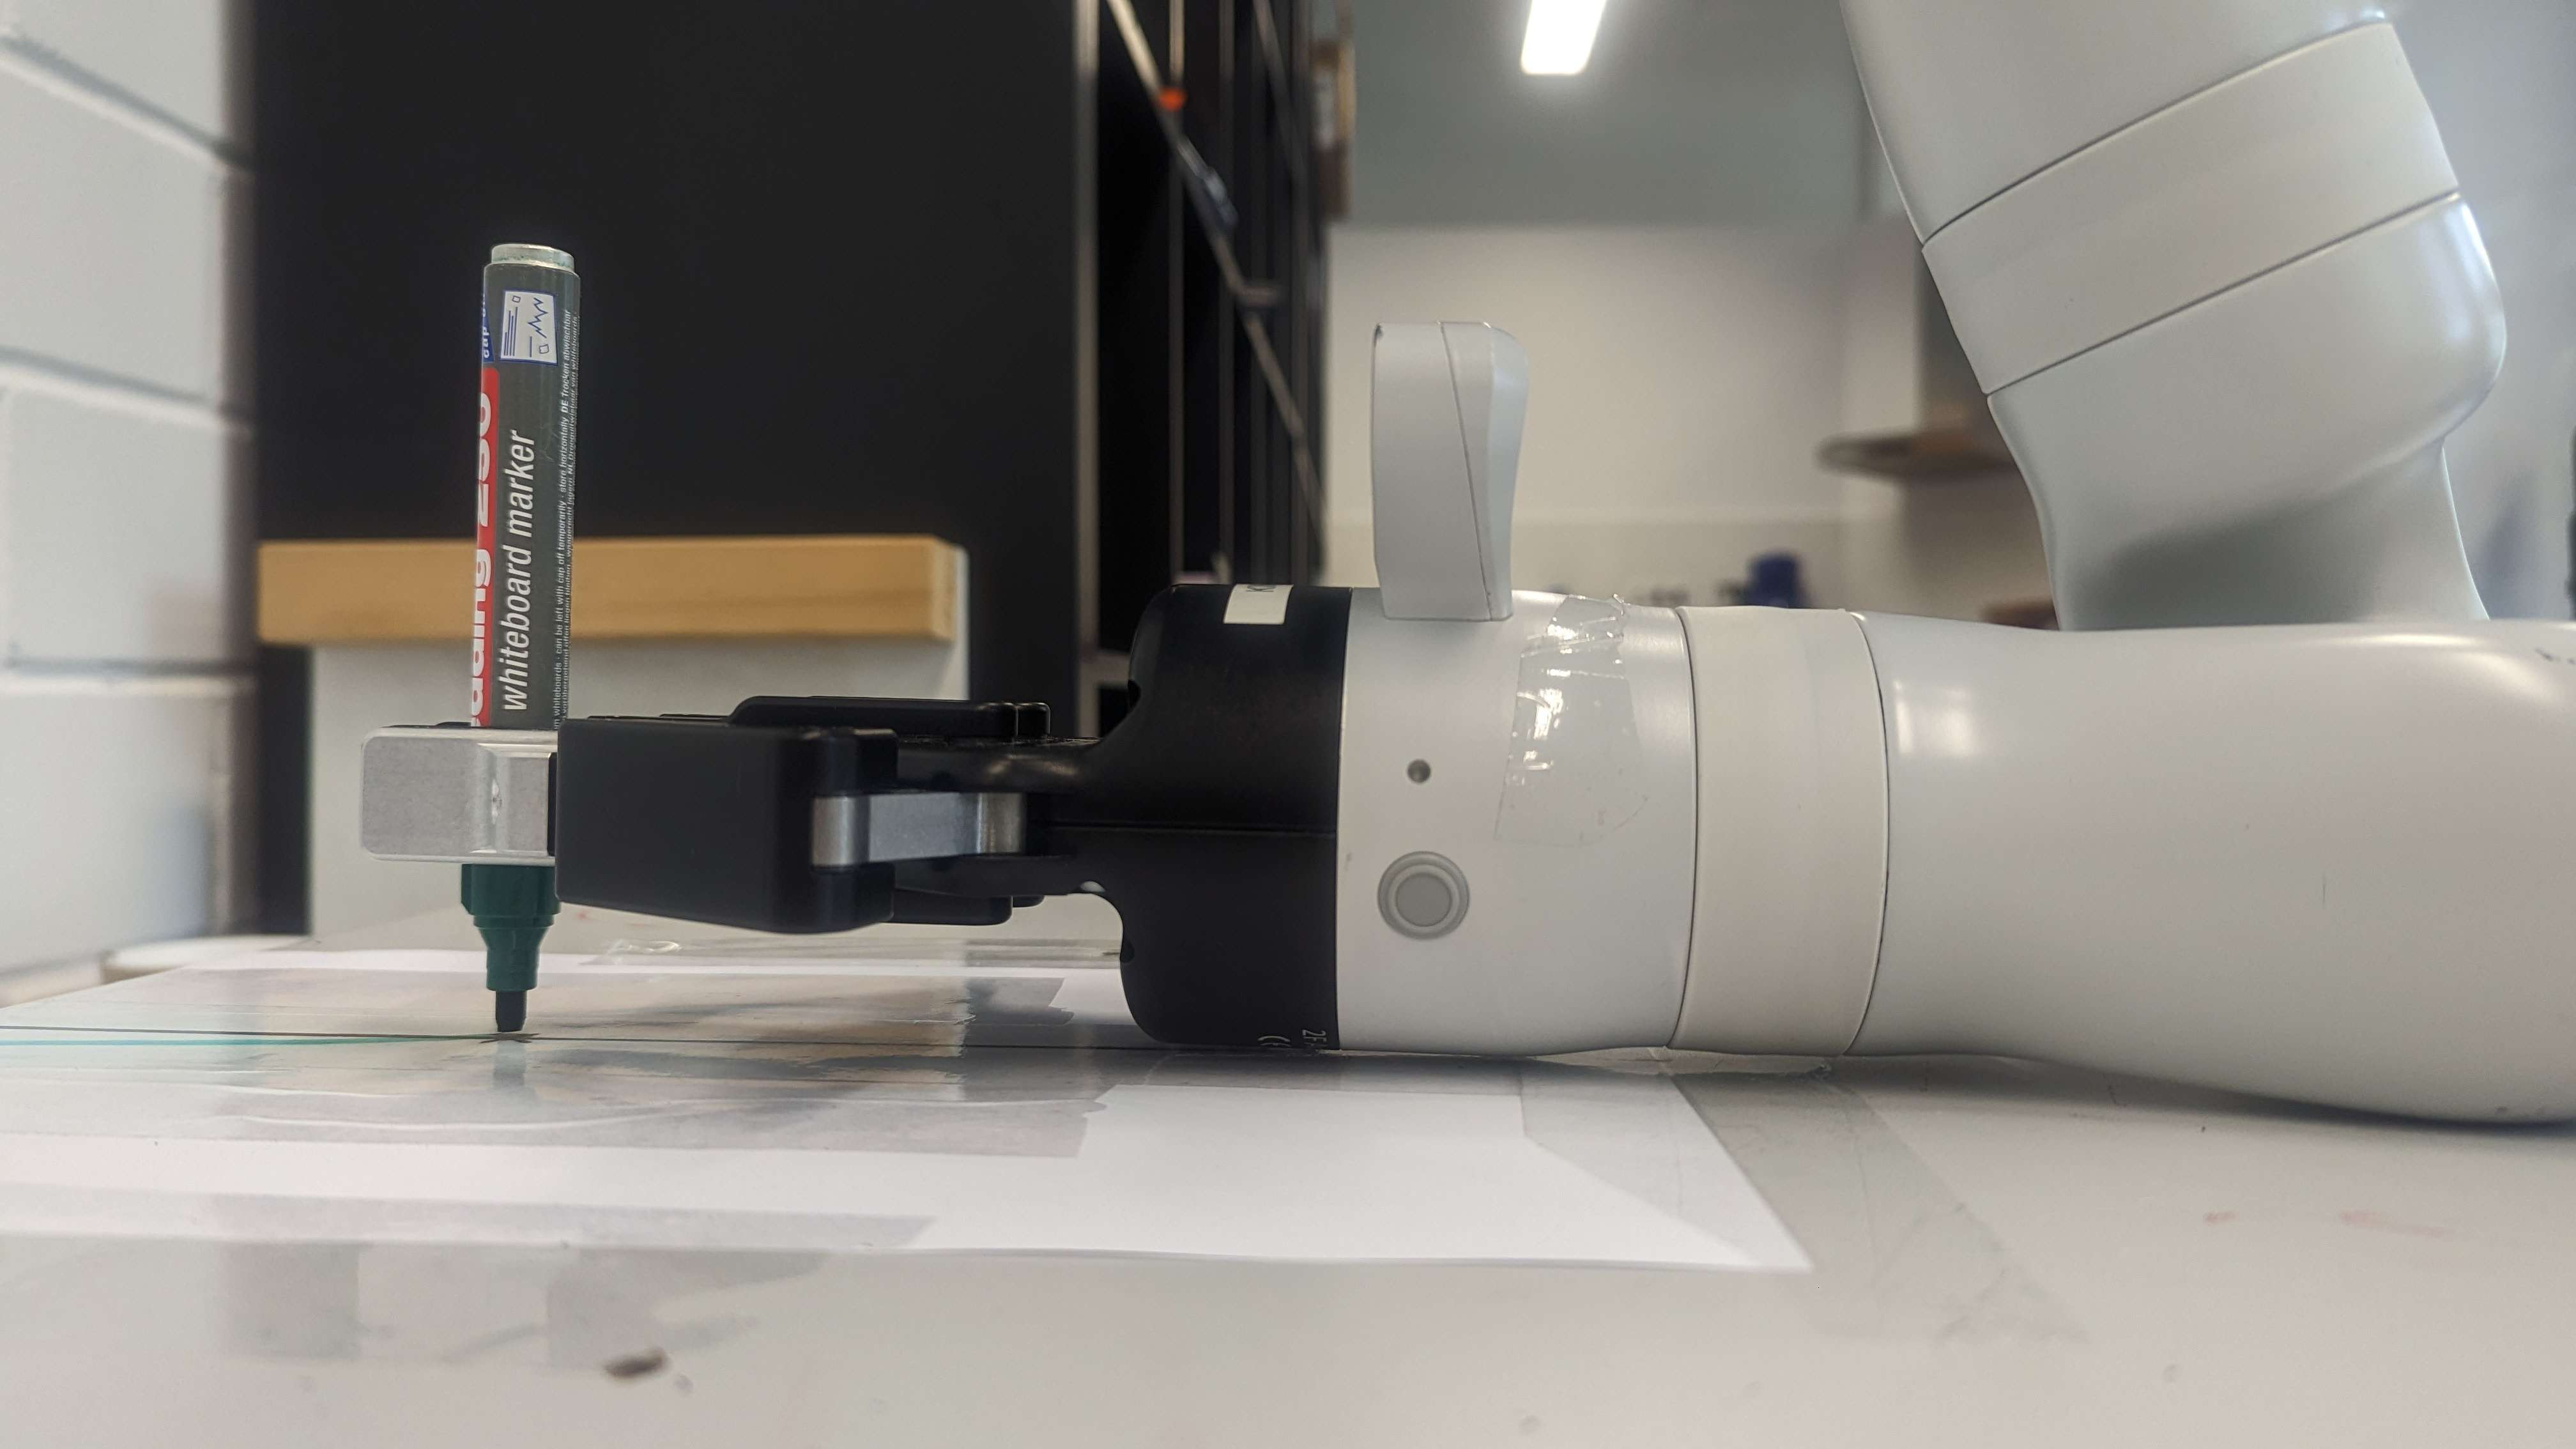
\includegraphics[width=\linewidth]{images/us2_contact.jpg}
            \caption{The initial pose of the robot arm of use case 2 in contact condition}
            \label{fig:us2_init_con}
        \end{subfigure}
        \begin{subfigure}{0.5\textwidth}
            \centering
            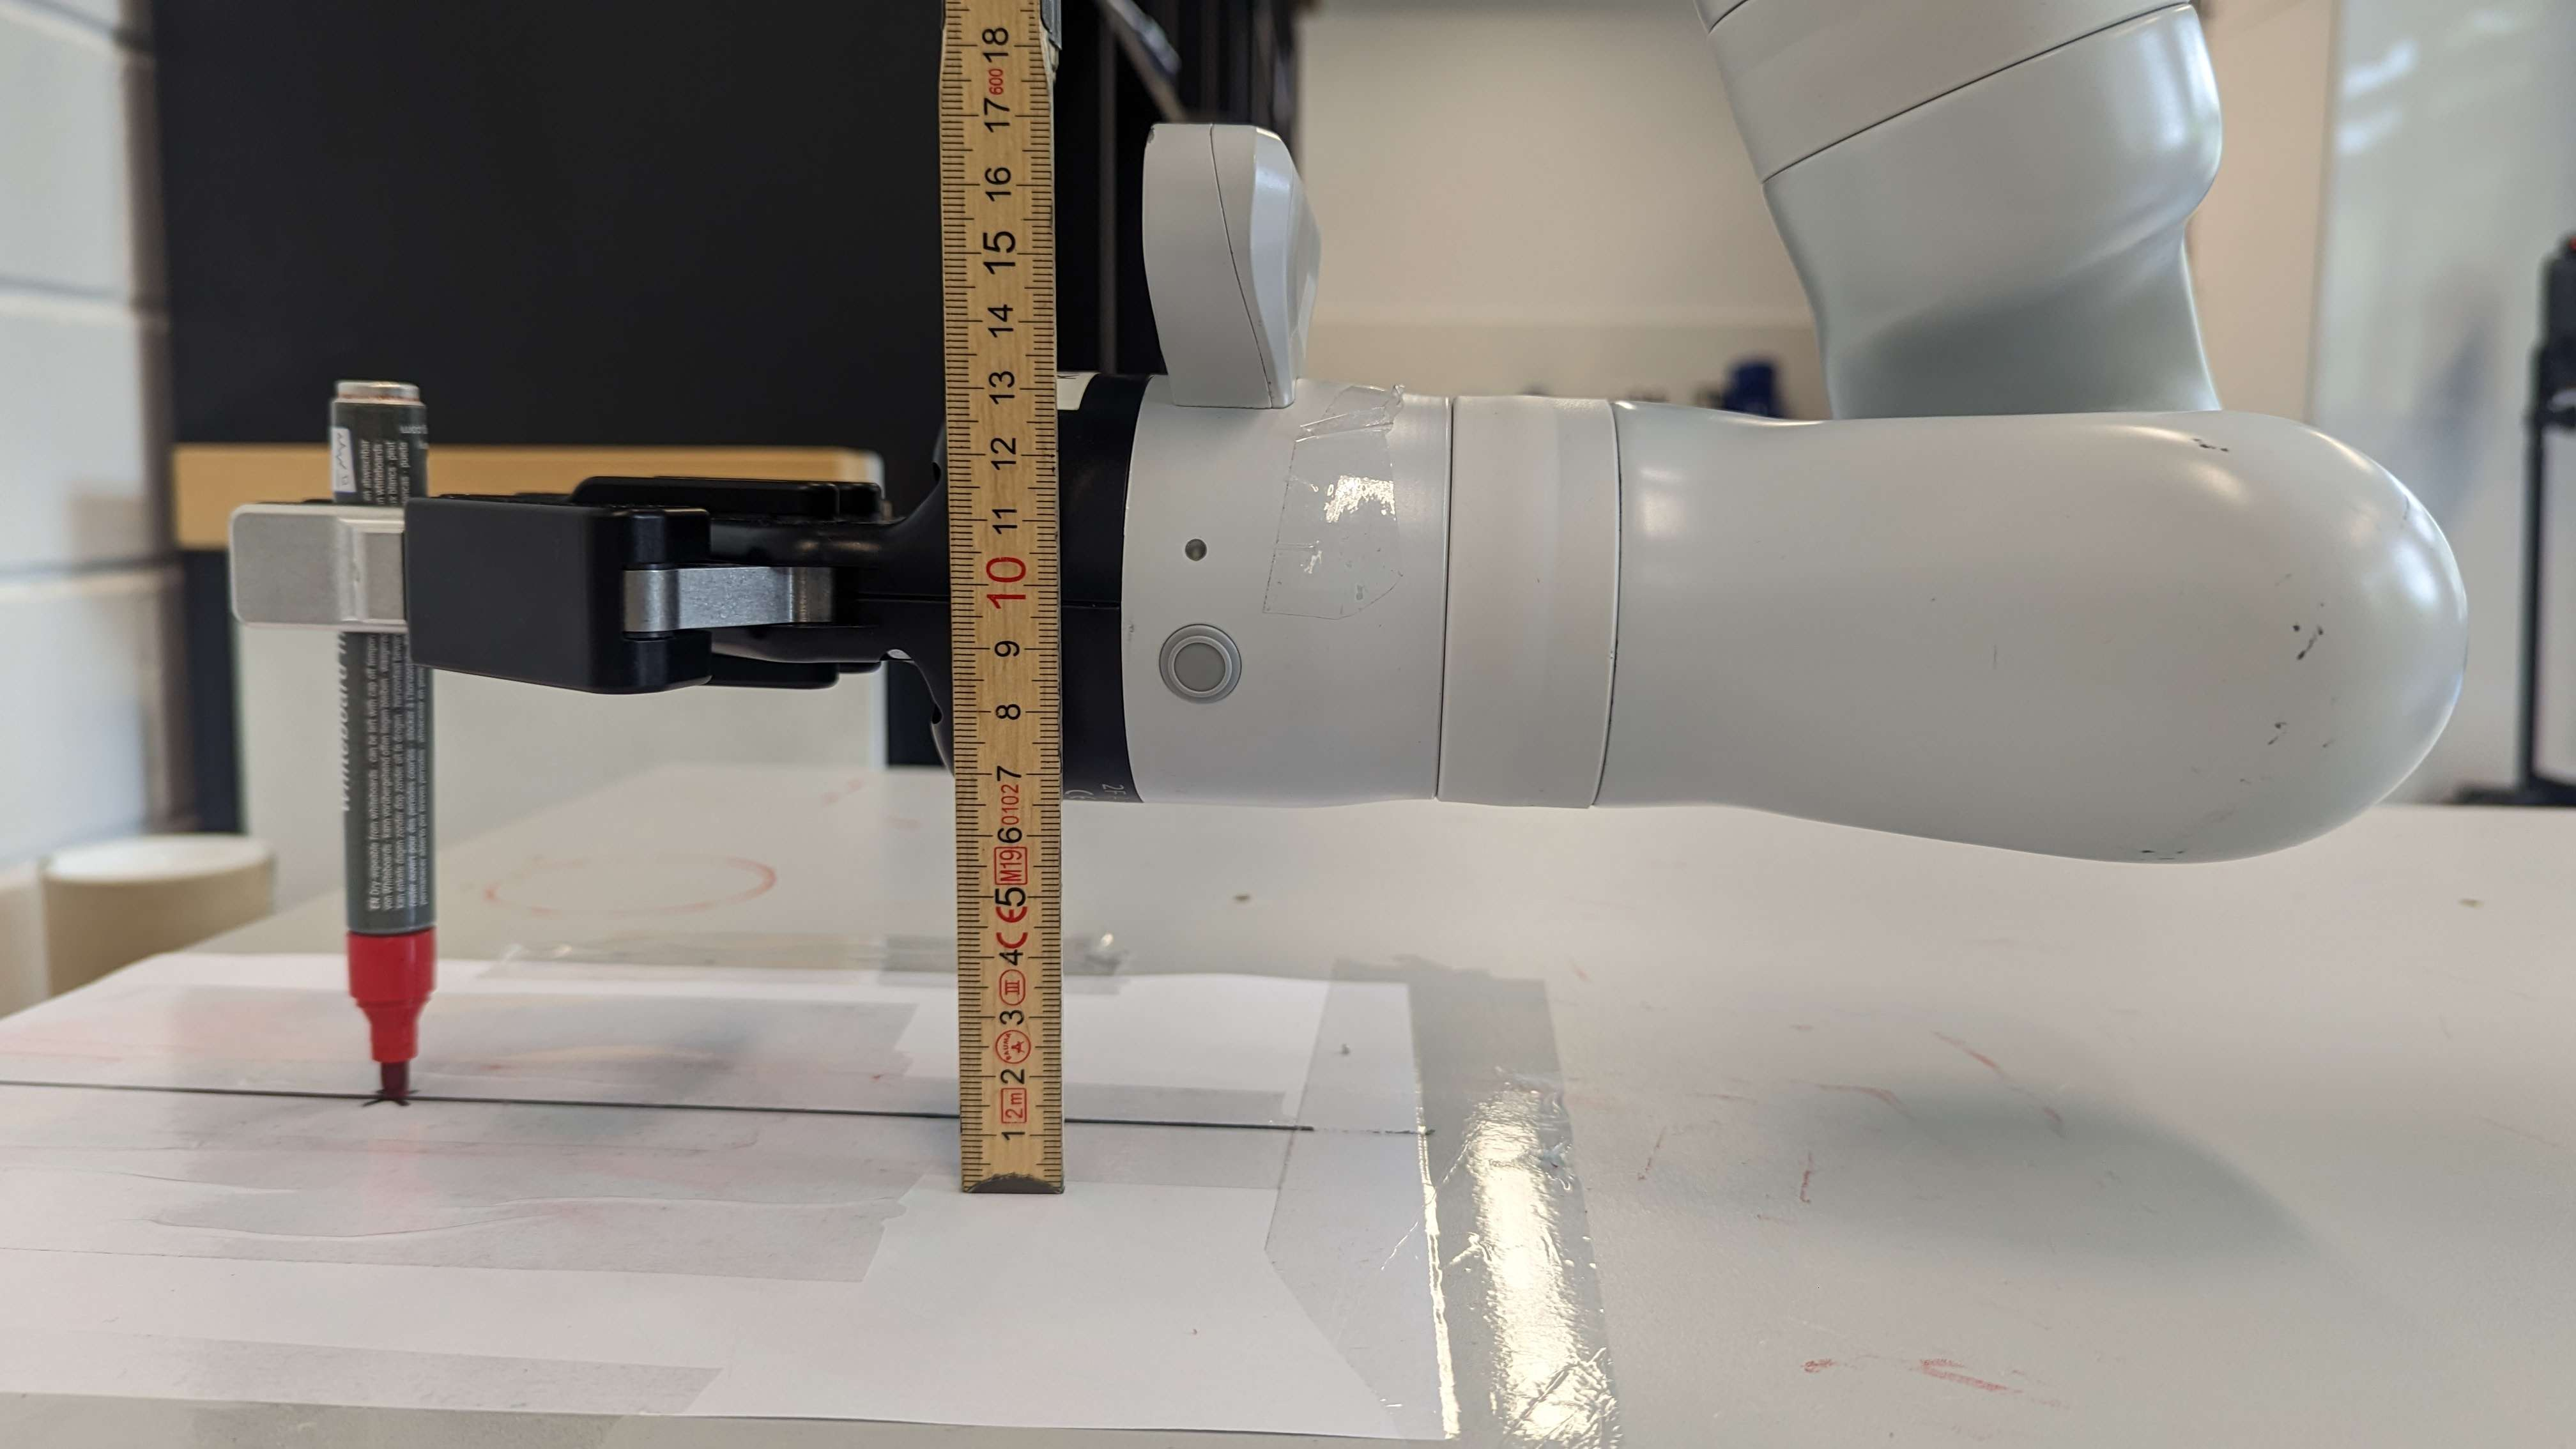
\includegraphics[width=\linewidth]{images/us2_nocontact.jpg}
            \caption{The initial pose of the robot arm of use case 2 in contactless condition}
            \label{fig:us2_init_nocon}
        \end{subfigure}
        \caption{initial position of use case 2}
\end{figure}

    \section{Use case 1 - Grasp object by sliding motion along surface} 
    The aim of this case study is to grasp the object successfully by sliding the robot
    manipulator along a contact surface. Assume that the object pose is known, 
    only the object to be grasped is on the table , no obstacle  and the contact surface is known.
    The manipulator should first approach the contact surface, for example, a table
    with the target object placed on it. When the manipulator is above the contact
    surface, it moves toward the surface until establishing contact. By activly monitoring the velocity along linear Z axis $v_{lin_z}$in world frame.
    If the absolute value of $v_{lin_z}$ for 10 samples is less than a threshold value. The contact between a surface and the robot manipulator is being established.
    After contact is established, the manipulator slides along the linear x direction for 10 cm $d_{x} = 0.1$ until it reaches a grasping
    region. Finally, the end-effector performs a grasping motion.


    \section{Use case 2 - Perform writing task} 
    The aim is to draw a line on the paper with a wrist joint contacting the writing
    surface like human writing. Before starting the manipulation task, the gripper
    firmly grasps the pen or marker. The manipulator should first approach the
    contact surface, for example, a table with the target object placed on it. When
    the manipulator is above the contact surface, it moves toward the surface until
    establishing contact. Once contact is established, the manipulator draws a line
    according to a predefined motion specification. The evaluation will be a trajectory
    comparison in terms of position or velocity with and without contact between the
    robot and the support surface
        \subsection{Setup}
        \subsection{Experimental Design}
        \begin{itemize}
            \item 
        \end{itemize}
    \section{Use case 3 - Resting elbow manipulation}
        \subsection{Experimental Design}
        \begin{itemize}
            \item 
        \end{itemize} 


%%%%
    % \chapter{Evaluation and Results}

    % \section{Experiment Description}

    % Describe the experiments/evaluation you are performing to analyse your method.

    % \section{Experimental Setup}  

    % Describe your experimental setup in detail.

    % \section{Results}

    % Describe the results of your experiments in detail.

\end{document}
